% Proxima v2 journal manuscript. Target: IEEE Transactions on Dependable
% and Secure Computing (IEEEtran journal mode); retargeting to another
% IEEE venue is a one-line class-option change.
\documentclass[journal]{IEEEtran}

\usepackage{amsmath,amssymb}
\usepackage{graphicx}
\usepackage{booktabs}
\usepackage{url}
\usepackage{cite}
\usepackage{microtype}

\graphicspath{{figures/}}

\newtheorem{theorem}{Theorem}
\newtheorem{lemma}{Lemma}
\newtheorem{corollary}{Corollary}
\newtheorem{proposition}{Proposition}
\newtheorem{definition}{Definition}

\newcommand{\dd}{\ensuremath{\Delta D}}
\newcommand{\norm}[1]{\ensuremath{\lVert #1 \rVert}}

\urldef{\repourl}\url{https://github.com/RyanMercier/Proxima}

\begin{document}

\title{Distance-Preserving Multiset Hashes: Separating Agreement
Estimation from Agreement Security in Byzantine Consensus}

\author{Ryan~Mercier%
\thanks{R. Mercier is with the School of Engineering, University of
Connecticut, Storrs, CT, USA (e-mail: ryan.mercier@uconn.edu).}%
\thanks{Code and reproduction artifacts: \repourl. An earlier version of this
work appeared at the 8th International Congress on Blockchain and
Applications~\cite{mercier2026proxima}; this article replaces that
version's primitive with a zero-mean construction, adds the binding
accumulator, the impossibility and composition theorems, robust reference
selection, readiness sensing, exact set reconciliation, and conservation
sharding, and evaluates against HotStuff-2 and Kauri.}}

\markboth{Preprint}{Mercier: Distance-Preserving Multiset Hashes}

\maketitle

\begin{abstract}
Byzantine fault tolerant (BFT) protocols compare validator state with
collision-resistant hashes, and collision resistance destroys distance:
validators that agree on 19 of 20 transactions produce unrelated hashes,
indistinguishable from validators that share nothing. We argue that
agreement \emph{estimation} and agreement \emph{security} are different
jobs that deserve different objects, and we show that one linear-algebraic
object can serve both. A distance-preserving multiset hash (DPMH) maps
each transaction to a zero-mean vector in $\{-1,+1\}^{n}$ and digests a
set by coordinate-wise integer summation, so that
$\norm{\dd}^{2}/n$ is an unbiased estimator of the multiset symmetric
difference with relative error at most $\sqrt{2/n}$, while equality of the
mod-$q$ digest is a collision-binding property whose violation reduces to
a short-integer-solution problem over a $\pm 1$ matrix. We prove that no
distance-preserving hash can make \emph{proximity} authoritative, which
forces an architecture: distance may gate scheduling, synchronization, and
optimism, never safety; and we prove a composition theorem showing that
any BFT protocol whose commit predicate is a quorum of signatures retains
its safety unchanged under such an estimation layer. On this foundation we
rebuild Proxima, a two-phase BFT protocol with a speculative fast path
whose trigger is honest-sufficient (a quorum of signed commitments, not a
variance statistic an adversary can perturb), a Byzantine-robust reference
(coordinate-wise median), straggler synchronization by
estimate-then-decode set reconciliation, $O(\log H)$ fork localization,
partition healing at cost proportional to divergence, and a cross-shard
\emph{conservation invariant} that verifies sharded settlement with
volume-independent metadata and localizes faulty corridors in
$O(f \log C)$ signed probes. Simulations confirm every closed form and
show the protocol consequences: a single in-cluster Byzantine validator
disables the prior fast path but not ours; a Byzantine aggregator excludes
every honest validator under the prior reference and none under ours; and
message complexity stays $1.5$ to $2\times$ below HotStuff-2 at
$N \le 3000$ while the bandwidth premium of kilobyte digests inverts in
our favor beyond $N \approx 2000$.
\end{abstract}

\begin{IEEEkeywords}
Byzantine fault tolerance, consensus, multiset hashing, sketching, set
reconciliation, sharding, blockchain.
\end{IEEEkeywords}

\IEEEpeerreviewmaketitle

%============================================================================
\section{Introduction}
\label{sec:intro}

\IEEEPARstart{B}{yzantine} fault tolerant consensus has been built on
collision-resistant hashing since PBFT~\cite{castro1999pbft}. Collision
resistance is the right property for preventing forgery and exactly the
wrong property for measuring agreement: when two validators hash their
transaction sets and the hashes differ, the protocol learns one bit, not
identical, whether the sets differ by one transaction or by half. Three
structural costs follow. Validators must synchronize state before they can
vote; agreement quality is unmeasurable until votes are counted, so
protocols such as HotStuff~\cite{yin2019hotstuff} run every voting round
even under unanimous agreement; and hierarchical designs need committees
large enough to run independent BFT, which is why Ethereum's attestation
committees hold 128 validators~\cite{eth2spec} and why cross-shard
transactions settle through per-transaction coordination.

The obvious repair, replacing the hash with a similarity-preserving
digest, runs into an equally obvious objection: a digest that maps nearby
sets to nearby values cannot be collision-resistant, so nothing it says
can be trusted against an adversary. Our starting point is that this
objection, made precise, is not a refutation but a design rule. We prove
that for \emph{any} distance-preserving multiset hash, digest proximity is
unbindable: an adversary can always exhibit sets within any threshold that
differ in ways a protocol cares about, because the distance property
itself guarantees it (Theorem~\ref{thm:impossible}). The conclusion is not
to abandon estimation but to route it away from safety. Estimation gates
\emph{scheduling}: when to propose, whom to synchronize, when to take an
optimistic path. Security remains what it always was: a quorum of
signatures on a collision-resistant hash. We formalize this separation and
prove it composes: any BFT protocol whose commit predicate is a signature
quorum retains its safety argument verbatim when an estimation layer is
added (Theorem~\ref{thm:compose}).

What makes the separation productive rather than merely safe is that a
single object serves both sides of it. Our distance-preserving multiset
hash (DPMH) digests a transaction multiset by summing per-transaction
Rademacher vectors, giving three properties no collision-resistant hash
offers: the squared digest distance is an unbiased estimator of the
multiset symmetric difference; digests add and subtract, so groups,
histories, and in-flight sets have exact one-object summaries; and the
same additive structure over a modulus is a homomorphic accumulator whose
equality is collision-binding under a short-integer-solution (SIS)
assumption, the algebra behind Ajtai hashing~\cite{ajtai1996sis} and
deployed in Facebook's LtHash~\cite{lewi2019lthash}. Estimation uses the
geometry; security uses only equality; the impossibility theorem says this
division of labor is forced, and the construction says it is cheap: one
SHA-512 and $n$ integer additions per transaction, one kilobyte on the
wire.

We rebuild the Proxima protocol of our conference
paper~\cite{mercier2026proxima} on this foundation and find that every
protocol mechanism sharpens:

\begin{itemize}
\item \textbf{Unbiased estimation (Sec.~\ref{sec:primitive}).} The
conference version used nonnegative coordinates, whose distance signal
depends on the direction of the difference: substituting $j$ transactions
reads at a fraction of its true size and can hide below honest stragglers.
Zero-mean coordinates measure exactly the symmetric difference
(Lemma~\ref{lem:unbiased}), the clustering threshold becomes the closed
form $\tau^{2} = 3n$ with honest-exclusion probability $e^{-n/8}$, and
Monte Carlo calibration is demoted to a validation check.
\item \textbf{Honest-sufficient fast path
(Sec.~\ref{sec:augment}).} Speculative signed commitments collected in
round one form a finality certificate identical to the slow-path object,
so the fast path is covered by the safety theorem verbatim; and because
the trigger counts signatures rather than testing a variance statistic,
one in-cluster Byzantine validator can no longer disable it. In
simulation the prior trigger's fast-path rate falls from 100\% to 0\% at
a single mimicking adversary; ours is unaffected
(Fig.~\ref{fig:fastpath}).
\item \textbf{Byzantine-robust reference (Sec.~\ref{sec:augment}).} The
clustering reference becomes the coordinate-wise median of the submitted
digests, verifiable by any validator, with breakdown point $1/2$ per
coordinate. Under a coordinated drag attack with a Byzantine aggregator,
the prior aggregator-chosen reference excludes 100\% of honest validators;
the median excludes none up to 45\% corruption (Fig.~\ref{fig:reference}).
\item \textbf{Readiness sensing (Sec.~\ref{sec:augment}).} Digests
piggybacked on gossip let the proposer measure convergence and propose
when a quorum already matches, converting fast-path engagement from
weather, $(1-p_{\mathrm{miss}})^{N}$, into a controlled quantity: at 80\%
initial miss rate, fixed-interval proposal never engages the fast path
and sensing engages it in every trial at a mean delay of $3.4$ gossip
ticks (Fig.~\ref{fig:fastpath}).
\item \textbf{Estimate-then-decode synchronization
(Sec.~\ref{sec:protocol}).} The digest distance sizes an invertible Bloom
lookup table~\cite{goodrich2011iblt} that recovers exactly the differing
transactions, replacing the conference version's Bloom filters and their
false-positive liveness channel. The same two-syndrome pattern heals
partitions at cost proportional to divergence and, with cumulative
accumulators, localizes chain forks in exactly $\log_{2} H + 1$ probes.
\item \textbf{Conservation sharding (Sec.~\ref{sec:conservation}).}
Cross-shard settlement becomes double-entry bookkeeping in vector space:
outbound and inbound corridor accumulators must sum to equality, a
collision-binding invariant checked with $O(S)$ kilobyte objects per
block regardless of volume. Violations are localized to faulty corridors
by group testing in $O(f \log C)$ signed probes and resolved exactly by
corridor syndromes: in a 16-shard run with 9 injected faults the
invariant's violation norm estimated $8.9$ dangling effects, aging alarms
and bisection named exactly the 2 faulty corridors in 15 probes, and the
decode recovered every dropped and minted transaction.
\end{itemize}

Sections~\ref{sec:related} through~\ref{sec:model} position and set up the
work; Sections~\ref{sec:primitive} and~\ref{sec:security} define the
primitive and its security envelope; Sections~\ref{sec:augment}
through~\ref{sec:conservation} build the protocol layer; and
Section~\ref{sec:eval} evaluates every claim against HotStuff,
HotStuff-2~\cite{malkhi2023hotstuff2}, Kauri~\cite{kauri}, and PBFT, with
the honest costs (a bandwidth premium at small $N$, a simulation-only
Kauri model, open cryptanalysis at exact parameters) stated where they
arise.

%============================================================================
\section{Related Work}
\label{sec:related}

\textbf{BFT consensus and speculation.} PBFT~\cite{castro1999pbft}
established practical BFT at $O(N^{2})$ messages;
HotStuff~\cite{yin2019hotstuff} reached linearity with leader-based
aggregation and threshold signatures, HotStuff-2~\cite{malkhi2023hotstuff2}
removed one of its three phases, and Tendermint~\cite{buchman2016tendermint}
offers a similar structure. All compare state by collision-resistant hash
and synchronize fully before voting. Our fast path descends from
speculative execution in Zyzzyva~\cite{kotla2007zyzzyva} and
SBFT~\cite{gueta2019sbft}, where optimistically collected signatures
finalize early when a large enough quorum already agrees; our contribution
is not the speculation but the estimation layer that decides when to
attempt it and the theorem that such layers cannot harm safety.

\textbf{Hierarchical and DAG designs.} Kauri~\cite{kauri} pipelines
tree-based dissemination and aggregation over HotStuff but keeps
per-group, hash-based voting, hence groups large enough for Byzantine
tolerance; Ethereum's 128-validator committees~\cite{eth2spec} exist for
the same reason. Distance filtering removes the per-group vote, so our
tree runs on groups of ten. Narwhal/Tusk~\cite{narwhal} and
Bullshark~\cite{bullshark} decouple data availability from ordering over
partial views; digests could measure vertex agreement there, which we
leave open.

\textbf{Multiset hashing and sketches.} Additive multiset hashes go back
to AdHash~\cite{bellare1997adhash}, broken into enormous moduli by
Wagner's generalized birthday attack~\cite{wagner2002gbp}, and were
formalized by Clarke et al.~\cite{clarke2003multiset}; the vectorized
form we use is deployed as LtHash~\cite{lewi2019lthash}, whose SIS-style
analysis~\cite{ajtai1996sis} we inherit. The estimation side is the
AMS/Tug-of-War sketch~\cite{ams1996} specialized to multiset indicator
vectors. What we add is the observation that one object carries both
properties at once, a quantitative adversarial-deflation analysis in the
public-hash setting with the two-domain design it forces, and the
consensus layer built on top. Hardt and Woodruff~\cite{hardt2013robust}
proved linear sketches are not robust to adaptive adversaries; our
impossibility theorem is the public-coin multiset-hash analogue, and our
composition theorem is the architectural answer. Locality-sensitive
hashing~\cite{indyk1998lsh,simhash,minhash,pstable} solves nearest
neighbors, not summable state comparison; we do not use it.

\textbf{Set reconciliation.} Exact reconciliation descends from
characteristic polynomials~\cite{minsky2003} through invertible Bloom
lookup tables~\cite{goodrich2011iblt}, Graphene~\cite{ozisik2019graphene},
minisketch as deployed in Bitcoin's Erlay~\cite{naumenko2019erlay}, and
rateless IBLTs~\cite{yang2024rateless}. Erlay is the existence proof that
set reconciliation belongs inside blockchain protocols; we generalize its
role from transaction relay to consensus synchronization, fork healing,
and cross-shard resolution, with the digest supplying the size estimate
that the decoder needs.

\textbf{Robust aggregation.} Coordinate-wise medians and trimmed means
with Byzantine breakdown guarantees come from robust distributed
learning~\cite{blanchard2017krum,yin2018robust}; we import them as
reference selection for clustering, which to our knowledge is new in
consensus.

\textbf{Sharding.} Ethereum moved to data-availability sharding
(Danksharding~\cite{danksharding}); NEAR's Nightshade~\cite{nightshade}
settles with receipts whose volume tracks transaction volume. Our
conservation invariant is complementary to both: constant-size settlement
verification with fraud localization, not an execution-ordering
mechanism.

%============================================================================
\section{System Model}
\label{sec:model}

We consider $N$ validators, at most $f < N/3$ Byzantine, behaving
arbitrarily and coordinating; honest validators follow the protocol. We
assume partial synchrony~\cite{dwork1988partialsync}: after an unknown
global stabilization time, messages between honest validators arrive
within a known bound. Each validator holds a BLS~\cite{boneh2004bls} key
pair with public keys known to all; signatures aggregate ($N$ signatures
into one 96-byte aggregate), and we assume CDH hardness in
BLS12-381~\cite{blst}. Communication runs through an aggregator (flat
mode) or a tree of relays (tree mode); the role rotates every round, and a
Byzantine aggregator can suppress messages, which costs liveness, but
cannot forge signatures. The adversary is static, corrupting validators
before the protocol begins; it observes the full network and may grind
transactions (Section~\ref{sec:security}). SHA-512 is modeled as a random
oracle. Honest validators may receive transactions with delay relative to
the proposer; $p_{\mathrm{miss}}$ denotes the per-validator probability of
an incomplete view at proposal time, and an incomplete honest view misses
at most $k_{\max} = 2$ transactions. Blocks are sets: multiplicity within
a block is bounded by one and enforced at validation.

%============================================================================
\section{The Primitive}
\label{sec:primitive}

\subsection{Construction}

For round (height) $h$, the per-transaction vector is
\begin{equation}
v_{h}(tx) \;=\; \mathrm{sgn}\bigl(H(\textsf{dom} \,\|\, h \,\|\,
tx)\bigr) \;\in\; \{-1,+1\}^{n},
\end{equation}
where $H$ is SHA-512, $\mathrm{sgn}$ maps each of the first $n$ output
bits $b$ to $2b - 1$, and $\textsf{dom}$ is a domain-separation tag. For
$n = 512$ one hash invocation suffices. The digest of a multiset $T$ is
the coordinate-wise integer sum
\begin{equation}
D_{h}(T) \;=\; \sum_{tx \in T} v_{h}(tx),
\end{equation}
stored as $n$ signed 16-bit words: each transaction moves each coordinate
by exactly one, so for any block with $|T| \le 32767$ the mod-$2^{16}$
encoding equals the integer digest with no wraparound. Homomorphism is
immediate in both directions, $D(A \uplus B) = D(A) + D(B)$ and
$D(A) - D(B)$ is meaningful, and group summaries travel as exact integer
pairs (sum of digests, total weight) so that no floating point ever
enters the protocol, eliminating cross-platform float nondeterminism as a
bug class. Computation is one SHA-512 plus $n$ integer additions per
transaction and one $O(n)$ dot product per distance.

Two domains coexist, and Section~\ref{sec:security} shows why both are
needed. \emph{Round digests} are salted by height ($\textsf{dom} =
\textsf{PXM/round}$, $q = 2^{16}$, $n = 512$) and feed clustering,
sensing, and synchronization. \emph{Ledger accumulators} use a fixed salt
($\textsf{dom} = \textsf{PXM/ledger}$, $q = 2^{32}$) and feed cumulative
chain digests $P[b] = \sum_{b' \le b} D(\text{block}_{b'})$, conservation
invariants, and fork localization, where equality must be binding and
algebra must compose across heights. Table~\ref{tab:params} lists the
profiles.

\begin{table}[t]
\caption{Parameter profiles. RSE is the relative standard error of the
symmetric-difference estimate; exclusion is the probability that an
honest validator with $d \le 2$ exceeds $\tau^{2} = 3n$.}
\label{tab:params}
\centering
\small
\begin{tabular}{@{}lrrrrl@{}}
\toprule
profile & $n$ & $q$ & wire & RSE & honest excl.\\
\midrule
round & 512 & $2^{16}$ & 1024\,B & $\le 6.3\%$ & $e^{-64}$\\
light & 128 & $2^{16}$ & 256\,B & $\le 12.5\%$ & $e^{-16}$\\
ledger & 512 & $2^{32}$ & 2048\,B & exact$^{\dagger}$ & n/a\\
\bottomrule
\end{tabular}
\vspace{2pt}

{\raggedright\footnotesize $^{\dagger}$Distance on accumulator
differences is exact below $q/2 = 2^{31}$ divergent transactions;
equality binding is unaffected by saturation.\par}
\end{table}

\subsection{Unbiased Distance Estimation}

Throughout this subsection the two multisets are fixed before the oracle
is queried; the adversarial regime is Section~\ref{sec:security}.

\begin{lemma}[Unbiased symmetric-difference estimator]
\label{lem:unbiased}
Let $d = |A \,\triangle\, B|$ and $\dd = D(A) - D(B)$. Then $\dd$ is
distributed as a sum of $d$ i.i.d.\ uniform $\{-1,+1\}^{n}$ vectors, and
\begin{equation}
\mathbb{E}\bigl[\norm{\dd}^{2}\bigr] = nd, \qquad
\hat{d} := \norm{\dd}^{2}/n \text{ is unbiased},
\end{equation}
with $\operatorname{Var}(\hat{d}) = 2d(d-1)/n$, hence relative standard
error at most $\sqrt{2/n}$ ($6.25\%$ at $n = 512$).
\end{lemma}

\begin{IEEEproof}
Vectors of elements in $A \cap B$ cancel in $\dd$; the remaining $d$
vectors appear with signs $\pm 1$, which the symmetry of the Rademacher
distribution absorbs. Per coordinate, $S = \sum_{i=1}^{d} \varepsilon_{i}$
with $\varepsilon_{i}$ i.i.d.\ Rademacher has $\mathbb{E}[S] = 0$,
$\mathbb{E}[S^{2}] = d$, and $\mathbb{E}[S^{4}] = 3d^{2} - 2d$. Summing
$\mathbb{E}[S^{2}]$ over $n$ independent coordinates gives
$\mathbb{E}\norm{\dd}^{2} = nd$; the variance of $\norm{\dd}^{2}$ is
$n(\mathbb{E}[S^{4}] - \mathbb{E}[S^{2}]^{2}) = n(2d^{2} - 2d)$, and
dividing by $n^{2}$ yields the claim.
\end{IEEEproof}

Two consequences shape the protocol. First, direction independence:
substituting $j$ transactions is a symmetric difference of $2j$ and is
measured as such, where the nonnegative coordinates of the conference
version~\cite{mercier2026proxima} let substitutions partially cancel and
read below honest stragglers. Second, exact small-$d$ laws that serve as
implementation test vectors: at $d = 1$, $\norm{\dd}^{2} = n$
deterministically (a singleton difference is certified by the exact value
$n$, with zero variance); at $d = 2$, $\norm{\dd}^{2} \sim 4\,
\mathrm{Bin}(n, 1/2)$; at $d = 3$, $\norm{\dd}^{2} \sim n + 8\,
\mathrm{Bin}(n, 1/4)$. Coordinates are independent, so Hoeffding also
gives the crude tail $\Pr[\,|\norm{\dd}^{2} - nd| \ge nt\,] \le
2\exp(-2nt^{2}/d^{4})$ for larger $d$.

\subsection{Closed-Form Threshold}
\label{sec:threshold}

An honest validator with an incomplete view misses at most $k_{\max} = 2$
transactions, so its digest sits at squared distance concentrated on
$nd \le 2n$ from the full-state digest. We therefore cluster at
\begin{equation}
\tau^{2} \;=\; 3n .
\end{equation}
Honest exclusion at $d = 2$ requires $4\,\mathrm{Bin}(n,1/2) > 3n$, i.e.,
a binomial deviation of $n/8$ above its mean, of probability at most
$e^{-n/8}$ ($e^{-64} \approx 1.6 \times 10^{-28}$ at $n = 512$); at
$d = 1$ exclusion is impossible since $n < 3n$. A fabrication at $d = 4$
sits $4.6$ standard deviations above the threshold. The value $d = 3$ is
genuinely ambiguous and is resolved by synchronization plus the signature
phase, never by the estimator; this ambiguity is inherent to any
finite-variance estimator and costs at most one round, never safety. The
conference version calibrated its threshold by Monte Carlo; here the
threshold is analytic and the simulation is only a validation check
(Section~\ref{sec:eval}).

%============================================================================
\section{Security of the Primitive}
\label{sec:security}

\subsection{Equality Binding}
\label{sec:binding}

A collision for the accumulator is a pair of distinct bounded-multiplicity
multisets with equal digests mod $q$, equivalently a nonzero integer
vector $z$ with bounded entries and bounded support such that $Vz \equiv 0
\pmod q$, where the columns of $V$ are the oracle-derived $\pm 1$ vectors
of the ground set. This is a short-integer-solution instance with a
$\pm 1$ matrix, the algebra of Ajtai hashing~\cite{ajtai1996sis} and of
LtHash~\cite{lewi2019lthash}. Collisions exist by pigeonhole, as they must
for any compressing homomorphic hash; security is the claim that finding
one is infeasible. Wagner's $k$-tree attack~\cite{wagner2002gbp} over
$\mathbb{Z}_{q}^{n}$ must cancel $n \log_{2} q = 8192$ constraint bits and
produces solutions of Hamming weight $2^{a}$ using lists of cost roughly
$2^{8192/(a+1)}$; the block-size cap $|T| \le 2^{15}$ forces $a \le 15$
and per-list cost $2^{512}$. Lattice attacks must find vectors in the
$q$-ary kernel lattice of $V$ far shorter than the Gaussian heuristic at
these parameters. We state binding as a reduction shape with these
first-cut estimates and inherit the parameter analysis of
LtHash~\cite{lewi2019lthash} at the same $n \log q$ budget; a dedicated
cryptanalysis at our exact parameters is open
(Section~\ref{sec:limits}), and we claim no concrete security level
without it.

\subsection{Adversarial Deflation and the Two Domains}
\label{sec:deflation}

Distance is an estimator, not a commitment, and a grinding adversary can
make a large true difference look smaller. The cheapest strategy is
near-antipodal pairs: for a target $v = v(tx)$, find $tx'$ whose vector
agrees with $-v$ on all but $a$ coordinates, so the pair contributes
$4a$ to the squared distance instead of the honest expectation $2n$.
Agreement counts are $\mathrm{Bin}(n, 1/2)$, so a pair achieving
$a \le n/4$ (factor-two deflation) occurs with probability
$e^{-n/8} = 2^{-92}$ at $n = 512$, and a birthday search over $M$
candidates yields about $M^{2} 2^{-93}$ usable pairs: one pair per
$2^{47}$ hash-and-sign candidates, each of which costs the adversary a
signable transaction. Factor-four deflation costs $2^{104}$ candidates
per pair. Deflation is therefore bounded to constant factors at
exponential grinding cost, and per-height salting of the round domain
forces any precomputed table to be rebuilt every block, converting a
one-time investment into an online per-block cost.

Salting, however, destroys cross-height algebra, which the accumulators
need. Hence the two domains of Section~\ref{sec:primitive}: the salted
round domain feeds thresholds, where deflation matters and no
cross-height algebra is needed; the fixed ledger domain feeds equality
and conservation checks, which rest on binding, not on distance, so
deflation is irrelevant there. Each domain carries exactly the property
it needs and no more.

\subsection{Proximity Is Unbindable}

\begin{theorem}[Proximity non-bindability]
\label{thm:impossible}
Let $D$ be any multiset hash with the distance-preservation property that
$|A \,\triangle\, B| \le d_{0}$ implies $\norm{D(A) - D(B)}$ small (below
any protocol threshold $\tau$) with non-negligible probability. Then
there is no security notion under which digest proximity certifies set
proximity against adversarially chosen inputs: for every threshold
$\tau$, the adversary can exhibit pairs of sets within $\tau$ that differ
in protocol-relevant ways. Consequently, in any protocol composed with
$D$, proximity may gate scheduling, synchronization, and optimistic
paths, but never a safety predicate.
\end{theorem}

\begin{IEEEproof}
For small differences the claim is the property itself: replace one
transaction by an adversarial one; distance preservation puts the
resulting set within $\tau$ for any usable $\tau$, and the sets differ in
exactly the transaction the adversary chose. For larger differences,
grinding (Section~\ref{sec:deflation}) extends the reach at quantifiable
cost, without ever needing a collision. Any protocol that commits state
on a proximity predicate therefore commits, with adversarial help, to a
set other than intended, violating safety by construction. The only
predicates immune to this argument are those independent of $D$'s
geometry, i.e., exact equality (Section~\ref{sec:binding}) and external
authentication such as signatures.
\end{IEEEproof}

Theorem~\ref{thm:impossible} is the public-coin, multiset-hash analogue
of the Hardt-Woodruff theorem that linear sketches are not robust to
adaptive inputs~\cite{hardt2013robust}. The resolutions differ: rather
than seeking a robust sketch, we route all safety through signatures on
collision-resistant hashes and let the estimator fail soft. The
conference version stated this honesty informally (``Phase 1 contributes
no cryptographic security''); the theorem makes the architecture forced
rather than stylistic.

%============================================================================
\section{Estimation-Augmented Consensus}
\label{sec:augment}

\begin{definition}[Estimation augmentation]
\label{def:augment}
Let $\Pi$ be a BFT protocol whose commit predicate is ``at least $2N/3$
valid signatures on $H(B)$'' for a collision-resistant $H$. An
\emph{estimation augmentation} $\Pi{+}E$ adds messages and rules that may
depend on DPMH digests, but whose outputs gate only scheduling (when to
propose, when to attempt a fast path), synchronization (which
transactions to push to whom), and reporting. The commit predicate is
unchanged.
\end{definition}

\begin{theorem}[Safety preservation]
\label{thm:compose}
$\Pi{+}E$ satisfies the same safety property as $\Pi$ against the same
adversary class.
\end{theorem}

\begin{IEEEproof}
Estimation messages are auxiliary: digests are computable from public
data and require no secrets. Given any adversary $\mathcal{A}$ against
$\Pi{+}E$, construct $\mathcal{A}'$ against $\Pi$ that internally
simulates the estimation layer, forwarding to $\Pi$ exactly the commit
messages $\mathcal{A}$ produces. The executions agree on all commit
messages, so any safety violation in $\Pi{+}E$ is one in $\Pi$. $\Pi$'s
safety argument, quorum intersection on signed $H(B)$, never invokes any
property of $D$.
\end{IEEEproof}

\begin{corollary}[Speculative fast path]
\label{cor:fastpath}
In Phase~1 each validator sends $(D_{i}, \sigma_{i})$ with $\sigma_{i}$ a
BLS signature on $(h, H(B_{\mathrm{prop}}))$, attached iff its local
state matches the proposal. If the aggregator collects $2N/3$ matching
signatures in round one, it aggregates them and multicasts a finality
certificate identical to the object the signature phase produces
(96-byte aggregate plus $N/8$-byte signer bitmap). The fast path is a
scheduling event under Definition~\ref{def:augment}, covered by
Theorem~\ref{thm:compose}; an aggregator cannot fabricate a certificate
and can at most withhold one, a liveness effect.
\end{corollary}

The corollary repairs two defects of the conference version at once. Its
fast-path certificate was issued from digest agreement alone, backed by
no signatures, which Theorem~\ref{thm:impossible} now rules out on
principle. And its trigger tested a global statistic, near-zero cluster
variance, which a single Byzantine validator inside the threshold could
perturb forever, disabling the fast path for free. Counting signatures is
\emph{honest-sufficient}: below the corruption bound the honest $2N/3$
match regardless of what the adversary submits. We state the design rule
explicitly because it generalizes: \emph{optimistic triggers must fire on
honest-sufficient conditions, never on global statistics the adversary
can perturb.}

\textbf{Robust reference.} The clustering reference in the conference
version was the aggregator's own state, a single manipulation point: a
Byzantine aggregator could place the reference anywhere and exclude every
honest validator. The reference is now the coordinate-wise median of the
submitted, signed Phase~1 digests, computable and verifiable by any
validator, with breakdown point $1/2$ per coordinate imported from robust
distributed learning~\cite{blanchard2017krum,yin2018robust}. A coalition
below one half cannot move any coordinate of the reference outside the
range of honest values, and the aggregator retains no discretion.

\textbf{Readiness sensing.} Because digests ride on gossip, the proposer
can watch the digest cloud converge and propose when the number of
exactly-matching validators reaches the quorum, rather than proposing on
a timer and hoping. Sensing turns the fast-path probability from the
weather term $(1 - p_{\mathrm{miss}})^{N}$ into a controlled quantity
bounded by gossip delay, at zero added messages (the observations ride
traffic that flows anyway); the cost is measured waiting time, which we
quantify in Section~\ref{sec:eval}.

\begin{theorem}[Liveness]
\label{thm:liveness}
Suppose $f < N/3$, each honest validator independently has an incomplete
view with probability $p_{\mathrm{miss}}$ missing at most $k_{\max} = 2$
transactions, and let $\delta_{\mathrm{sync}}$ bound the probability that
a flagged straggler fails to synchronize before the signature-phase
timeout. Then the per-honest-validator probability of failing to
contribute a signature is $p \le p_{\mathrm{miss}} e^{-n/8} +
\delta_{\mathrm{sync}}$, and consensus fails to finalize with probability
at most $\exp\!\bigl(-2N(1/3 - p)^{2}\bigr)$.
\end{theorem}

\begin{IEEEproof}
An honest validator misses a signature only if falsely excluded
(probability at most $e^{-n/8}$ conditioned on an incomplete view, by the
threshold analysis of Section~\ref{sec:threshold}) or unsynchronized.
Exclusions are independent across validators; Hoeffding over the $N$
honest indicators against the $N/3$ failure boundary gives the bound.
\end{IEEEproof}

At $n = 512$ the false-exclusion term is $p_{\mathrm{miss}} e^{-64}$,
negligible against $\delta_{\mathrm{sync}}$; liveness is governed by the
synchronization path, as it should be. The conference version's
false-exclusion term was an empirical $5 \times 10^{-3}$; the analytic
replacement is twenty-six orders of magnitude smaller, and exclusion is
now a scheduling event rather than a participation event, since a synced
straggler rejoins the signature phase.

%============================================================================
\section{The Proxima Protocol}
\label{sec:protocol}

\textbf{Flat protocol.} The proposer disseminates the block; validators
receive it with delay $p_{\mathrm{miss}}$. In Phase~1 each validator
sends its round digest (1024\,B) and, if its state matches, the
conditional commitment $\sigma_{i}$ (96\,B). The aggregator forms the
median reference, clusters by the integer comparison
$\norm{\dd}^{2} \le 3n$, and synchronizes stragglers by
estimate-then-decode: the digest distance sizes an IBLT whose peeling
returns exactly the missing transactions, which the aggregator then
pushes. With $2N/3$ commitments in hand the fast path finalizes in one
round trip (Corollary~\ref{cor:fastpath}); otherwise cluster members send
signed commitments and the aggregator multicasts the aggregate plus
bitmap. Every decision on the consensus path is an integer comparison.

\textbf{Tree protocol.} Validators form leaves of ten; leaf leaders
filter by distance, synchronize stragglers, and forward the exact summary
(digest sum, weight, squared-distance sum, 1036\,B); internal nodes add
summaries, which is exact by linearity, and the root checks the global
mean. The signature phase aggregates BLS commitments up the tree. Leaves
never vote, so no leaf can fail in the BFT sense: a leaf of five honest
and five Byzantine validators reports the filtered mean of the honest
five. Carrying speculative commitments up the tree requires per-group
signer bitmaps and remains future work.

\textbf{Two-syndrome synchronization.} The digest is the syndrome of a
random linear code over $\mathbb{Z}_{q}$: hard to decode, which is
exactly the binding of Section~\ref{sec:binding}, but with error weight
estimable from the syndrome norm (Lemma~\ref{lem:unbiased}). IBLTs are
the complementary syndrome: efficiently decodable, recovering the exact
difference at communication proportional to it, but neither binding nor
distance-revealing. The protocol always pairs them: estimate with the
hard code, decode with the easy one, at IBLT size $1.5(\hat{d} + 6)$
cells of 16 bytes, doubling on the rare decode failure. This replaces the
conference version's Bloom filters everywhere and deletes their
false-positive liveness channel outright, since IBLT peeling has no false
positives.

\textbf{Fork localization and partition healing.} Cumulative ledger
accumulators make any range digest a subtraction, so two nodes locate
their fork point by binary search on prefix equality: $\log_{2} H + 1$
probes of one accumulator each, with every probe also yielding
$\hat{d}$ for the probed range, after which one reconciliation exchange
heals the divergent suffix. During a partition the Phase~1 cloud turns
bimodal; cluster centroids are exact by linearity, the inter-camp
$\hat{d} = \norm{\mu_{1} - \mu_{2}}^{2}/n$ measures the disagreement
before any repair traffic flows, and one estimate-then-decode exchange
between camp representatives restores the union at cost proportional to
the true divergence. Hash-based protocols observe only quorum failure in
both situations. The same subtraction gives verifiable prune accounting:
a node claiming to have pruned set $P$ proves $D(\text{before}) -
D(\text{after}) = D(P)$, and binding makes the claim sound.

%============================================================================
\section{Cross-Shard Conservation}
\label{sec:conservation}

Sharded execution multiplies state comparison into many pairs, and
hash-based tools force per-transaction coordination: two-phase commit
spends four cross-shard messages per transaction plus intra-shard
consensus on each, and receipt systems~\cite{nightshade} carry metadata
proportional to volume. We instead make settlement a conservation law.
Every cross-shard transaction $t$ from shard $i$ to shard $j$ adds
$v(t)$ (ledger domain) to $i$'s outbound corridor accumulator
$O_{i \to j}$ when the debit applies and to $j$'s inbound accumulator
$I_{i \to j}$ when the credit applies; each shard's quorum signs its
aggregated outbound and inbound accumulators every block, and the beacon
checks
\begin{equation}
\textstyle\sum_{i} O_{i} \;=\; \sum_{j} I_{j}
\end{equation}
over a settlement window $W$: double-entry bookkeeping in vector space,
at $O(S)$ kilobyte-scale signed objects per block regardless of volume.

\begin{theorem}[Conservation soundness]
\label{thm:conservation}
If the invariant holds over quorum-signed accumulators and the
accumulator is collision-binding, then the multiset of applied debits
equals the multiset of applied credits except with negligible
probability; any minted, lost, or replayed cross-shard effect requires
forging a quorum signature or finding a digest collision.
\end{theorem}

\begin{IEEEproof}
The invariant asserts $D(\text{debits}) = D(\text{credits})$ in the
ledger domain. If the underlying multisets differ, the pair is a
collision (Section~\ref{sec:binding}); if a shard signs an accumulator
inconsistent with its applied transactions, safety of its intra-shard
quorum is violated. Value conservation follows from multiset conservation
plus intra-shard execution validity, since amounts are bound inside the
hashed transactions; we deliberately do not weight vectors by amounts,
which would weaken the SIS instance.
\end{IEEEproof}

\begin{proposition}[Localization by group testing]
\label{prop:localize}
On invariant failure, the beacon bisects the corridor set with digests
aggregated over halves, recursing into imbalanced halves. Bisection over
a linear measurement is exact, and $f$ faulty corridors among $C$ are
localized in at most $2f(\log_{2}(C/f) + 2)$ probes, each one signed
kilobyte-scale object.
\end{proposition}

Two refinements make the mechanism operational. First, the per-corridor
\emph{pending digest} $P_{ij} = O_{i \to j} - I_{i \to j}$ is not merely
an alarm signal: it is the ledger digest of the in-flight transaction set
on that corridor, so its norm meters in-flight volume continuously, and
the invariant is enforced as ``$P_{ij}$ decays to zero within $W$
blocks,'' with aging alarms separating ordinary settlement lag from
faults, since credits necessarily trail debits by network latency.
Second, each corridor can carry the IBLT syndrome of the same in-flight
set alongside $P_{ij}$ (both objects are linear), so an alarmed corridor
decodes exactly its dangling transactions, dropped credits and minted
credits alike, from the source's applied-debit set against the
destination's applied-credit set, with no further exchange.

The semantics deserve a plain statement: this is detection and settlement
verification, not locking. Digests order nothing; the protocol pairs the
invariant with optimistic execution and a $W$-block revert window, or
credits at the destination only on digest match, which is
receipt-equivalent in latency but constant-size in verification metadata.
The contribution is the verification and fraud-localization cost, and the
fair baseline comparison is per-block verification metadata against
batched two-phase commit and batched receipts, which we report in
Section~\ref{sec:eval}. A beacon may additionally maintain the single
running digest $G \mathrel{+}= \sum_{i} \Delta_{i}$ per block, one 2\,KB
object summarizing the entire system's applied history, updatable by
addition and prunable by subtraction with verifiable prune accounting,
none of which a Merkle root supports.

%============================================================================
\section{Evaluation}
\label{sec:eval}

All experiments run in the discrete-event simulator of the public
artifact, which counts every message with identical byte constants across
protocols; BLS operations use mocks preserving wire sizes, cross-validated
against real BLS12-381 on small runs. The suite of 41 correctness checks,
including the exact test vectors of Section~\ref{sec:primitive}, passes
on every run reported here. Baselines are HotStuff~\cite{yin2019hotstuff},
HotStuff-2~\cite{malkhi2023hotstuff2}, PBFT~\cite{castro1999pbft}, and a
message-count model of Kauri~\cite{kauri} (fanout 10) that credits its
tree dissemination but not its pipelining and does not charge its
reconfiguration on relay failure, a deliberately generous simplification
we return to below. Unless stated, $N$ splits 70/30 honest/Byzantine,
$p_{\mathrm{miss}} = 0.37$ with $k_{\max} = 2$, and blocks carry 21
transactions.

\subsection{The Estimator Behaves as Proved}

Fig.~\ref{fig:estimator} shows $\norm{\dd}^{2}/n$ against ground truth
for missing and substituted transactions: samples collapse onto the
analytic line $\hat{d} = d$, the $d = 1$ case is exactly $n$ with zero
observed variance across 400 trials, and substitutions read their full
symmetric difference, closing the conference version's blind spot.
Fig.~\ref{fig:threshold} plots the exact small-$d$ laws against
$\tau^{2} = 3n$: $d \le 2$ sits cleanly below threshold ($0$ exclusions
in 500 validation trials, against the $e^{-64}$ bound), $d = 4$ cleanly
above, and $d = 3$ straddles it, resolved by synchronization as designed.

\begin{figure}[t]
\centering
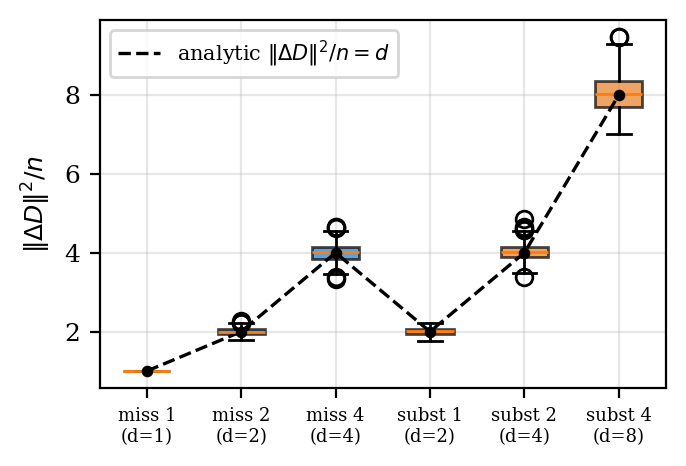
\includegraphics[width=\columnwidth]{fig1_estimator.png}
\caption{Squared digest distance over $n$ against true symmetric
difference, for missing (blue) and substituted (orange) transactions,
400 trials per case at $n = 512$. Boxes collapse onto the analytic line;
$d = 1$ has zero variance.}
\label{fig:estimator}
\end{figure}

\begin{figure}[t]
\centering
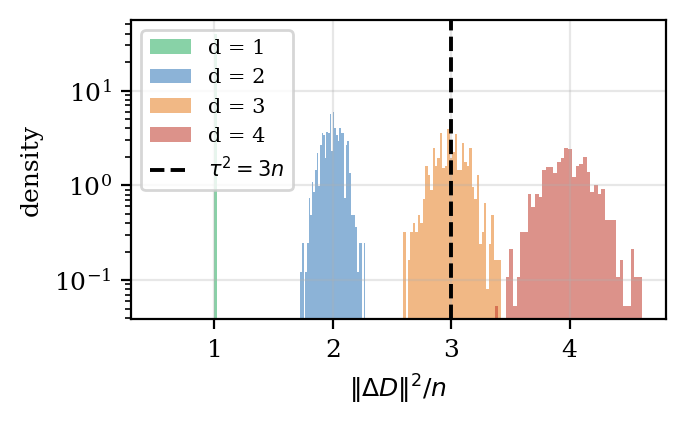
\includegraphics[width=\columnwidth]{fig2_threshold.png}
\caption{Distributions of $\norm{\dd}^{2}/n$ at $d = 1, \dots, 4$ against
the closed-form threshold $\tau^{2} = 3n$ (log scale). $d = 1$ is a point
mass at exactly $1$; honest stragglers ($d \le 2$) never cross the
threshold; $d = 3$ is the designed ambiguity region.}
\label{fig:threshold}
\end{figure}

\subsection{Reference Robustness}

Fig.~\ref{fig:reference} mounts a coordinated drag attack: all Byzantine
validators submit one extreme digest and the aggregator is itself
Byzantine. With the conference version's aggregator-chosen reference the
adversary excludes 100\% of honest validators at every corruption level,
a total liveness failure available to a single corrupted role. The
coordinate-wise median reference excludes no honest validator up to the
45\% corruption we tested, matching its breakdown guarantee.

\begin{figure}[t]
\centering
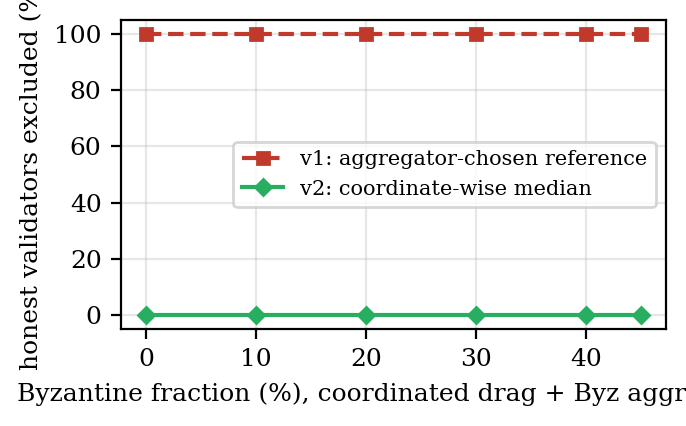
\includegraphics[width=\columnwidth]{fig3_reference.png}
\caption{Honest exclusion under coordinated drag with a Byzantine
aggregator, $N = 90$, eight trials per point. The aggregator-chosen
reference (v1) admits total exclusion; the coordinate-wise median (v2)
admits none through 45\% corruption.}
\label{fig:reference}
\end{figure}

\subsection{Fast Path: Griefing and Sensing}

Fig.~\ref{fig:fastpath} (left) is the griefing experiment: mimicking
Byzantine validators sit inside the cluster and perturb its variance. The
variance trigger of the conference version drops from 100\% to 0\%
fast-path engagement at a single such adversary and never recovers; the
commitment-counting trigger is indifferent through eight, as
honest-sufficiency predicts. Fig.~\ref{fig:fastpath} (right) evaluates
readiness sensing at increasing initial miss rates with a gossip fill
probability of $0.5$ per tick and an 8-tick cap: fixed-interval proposal
collapses to a 6\% fast-path rate at $p_{\mathrm{miss}} = 0.2$ and to
zero beyond $0.4$, while the sensing proposer waits a measured mean of
$1.3$ to $3.4$ ticks and engages the fast path in every trial through
$p_{\mathrm{miss}} = 0.8$. Sensing spends bounded, observable delay to
buy a round; the exchange rate is the gossip fill time, not a protocol
constant.

\begin{figure*}[t]
\centering
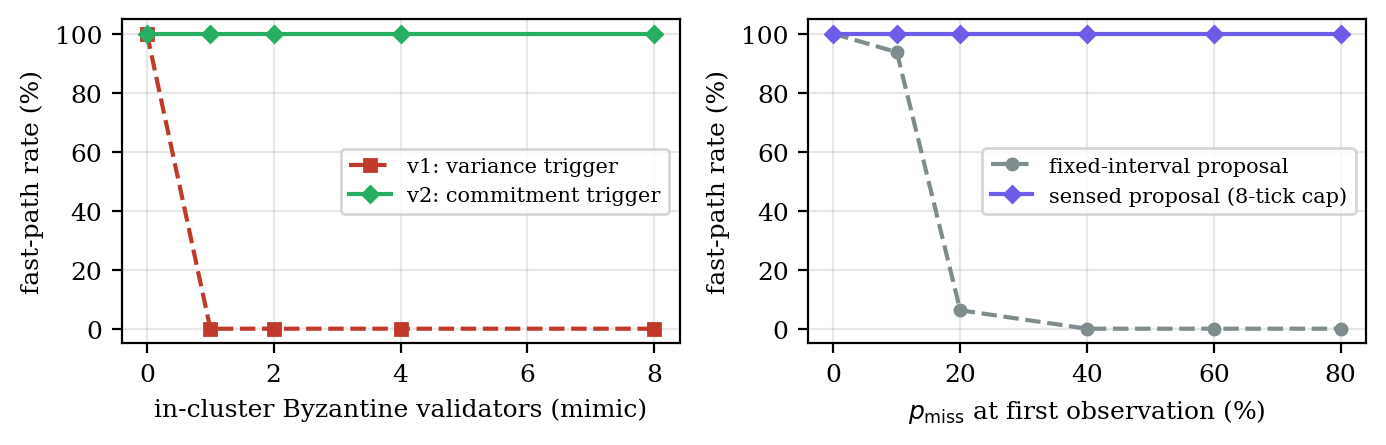
\includegraphics[width=\textwidth]{fig4_fastpath.png}
\caption{Left: fast-path rate against in-cluster mimicking Byzantine
validators ($N = 60$ honest, complete views); the variance trigger dies
at one adversary, the commitment trigger is unaffected. Right: fast-path
rate against initial $p_{\mathrm{miss}}$ for fixed-interval versus sensed
proposal (fill probability $0.5$ per tick, cap 8 ticks, mean measured
delay $0$ to $3.4$ ticks).}
\label{fig:fastpath}
\end{figure*}

\subsection{Synchronization Cost}

Fig.~\ref{fig:sync} compares straggler synchronization sketches at local
set size 500. The Bloom filter of the conference version costs a flat
599 bytes because it encodes the whole set, and carries a false-positive
channel besides; the IBLT costs 256 bytes up to $d = 4$ and grows
linearly in the true difference with exact decode (every trial decoded in
one round at the estimator-supplied size). Below $d \approx 16$ the exact
sketch is also the cheaper one; beyond, it pays only for what actually
differs.

\begin{figure}[t]
\centering
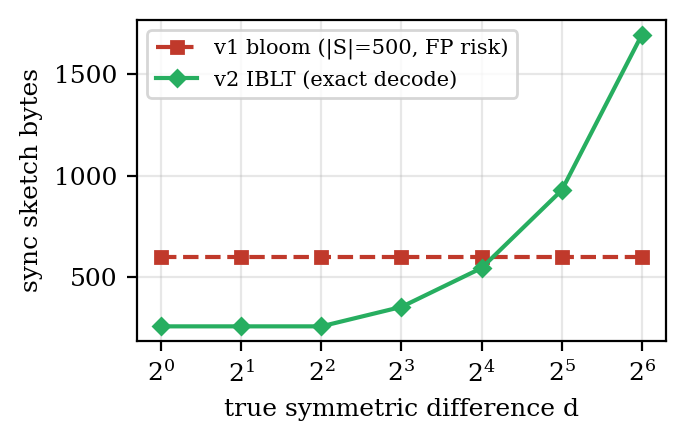
\includegraphics[width=\columnwidth]{fig5_sync.png}
\caption{Sync sketch bytes against true difference at set size 500. The
Bloom filter scales with the set and admits false positives; the IBLT
scales with the difference and decodes exactly.}
\label{fig:sync}
\end{figure}

\subsection{Conservation}

Fig.~\ref{fig:conservation} (left) plots per-block verification metadata
at $S = 16$ shards: batched receipts and batched two-phase commit grow
with volume, conservation is flat at 67\,KB, and the crossover sits at
roughly 2{,}100 cross-shard transactions per block, below which receipts
are cheaper and above which conservation wins unboundedly.
Fig.~\ref{fig:conservation} (right) confirms
Proposition~\ref{prop:localize}: measured localization probes at $C = 64$
corridors track $2f(\log_{2}(C/f) + 2)$ and localization was exact in
every run. The end-to-end fault run of Section~\ref{sec:conservation}
(16 shards, 14{,}400 transactions, 9 injected faults across two
corridors, one of them a minted credit) detected the violation with a
dangling-effect estimate of $8.9$ against the true 9, named exactly the
two faulty corridors both by aging alarms and by 15 bisection probes, and
the corridor syndrome decode recovered every dropped and minted
transaction exactly.

\begin{figure*}[t]
\centering
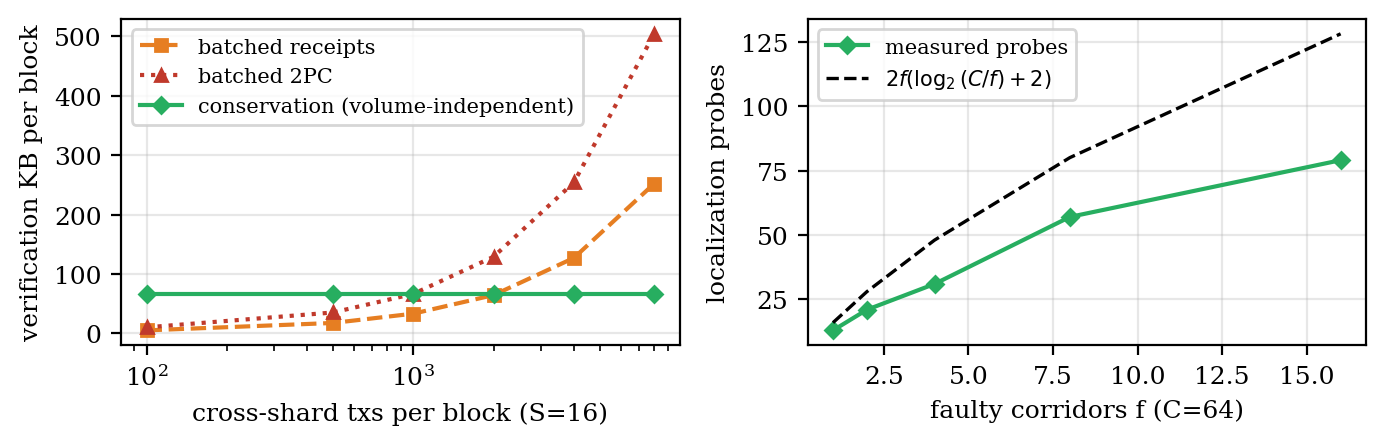
\includegraphics[width=\textwidth]{fig6_conservation.png}
\caption{Left: per-block verification metadata at $S = 16$; conservation
is volume-independent, with the receipts crossover near 2{,}100
cross-shard transactions per block. Right: localization probes against
faulty-corridor count at $C = 64$, with the analytic budget.}
\label{fig:conservation}
\end{figure*}

\subsection{Scaling Against Modern Baselines}

Fig.~\ref{fig:scaling} and Table~\ref{tab:scaling} give message and
bandwidth scaling to $N = 3000$ with 30\% Byzantine and 37\% partial
observation. On messages, Proxima Tree runs $1.99\times$ below HotStuff
and $1.69\times$ below HotStuff-2 at $N = 3000$, with the Kauri model
above flat HotStuff since tree dissemination adds edges without removing
voting; the conference version's headline held only against three-phase
HotStuff, and this is the corrected claim. On bandwidth the picture
inverts and is worth stating carefully: kilobyte digests make Proxima
$1.4$ to $1.6\times$ heavier than HotStuff-2 at $N \le 300$, the gap
closes through $N = 1000$, and beyond $N \approx 2000$ Proxima is
lighter, because certificate bitmaps broadcast to all validators cost
the hash-based protocols $\Theta(N^{2}/8)$ bytes while digests cost
$\Theta(N)$. Deployments below the crossover can take the light profile
(256-byte digests at 12.5\% estimator error, Table~\ref{tab:params});
we report the default profile throughout.

\begin{table}[t]
\caption{Messages and KB per block (30\% Byzantine,
$p_{\mathrm{miss}} = 0.37$).}
\label{tab:scaling}
\centering
\footnotesize
\begin{tabular}{@{}lrrrr@{}}
\toprule
 & \multicolumn{2}{c}{$N = 1000$} & \multicolumn{2}{c}{$N = 3000$}\\
\cmidrule(lr){2-3}\cmidrule(lr){4-5}
protocol & msgs & KB & msgs & KB\\
\midrule
Proxima Tree & 3{,}286 & 1{,}506 & 9{,}818 & 5{,}103\\
Proxima Flat & 3{,}644 & 1{,}415 & 10{,}884 & 4{,}742\\
HotStuff & 6{,}518 & 1{,}322 & 19{,}554 & 6{,}164\\
HotStuff-2 & 5{,}518 & 1{,}195 & 16{,}554 & 5{,}782\\
Kauri (msg model) & 7{,}511 & 1{,}105 & 22{,}547 & 4{,}297\\
PBFT & 1{,}999{,}000 & 249{,}875 & 17{,}997{,}000 & 2{,}249{,}625\\
\bottomrule
\end{tabular}
\end{table}

\begin{figure*}[t]
\centering
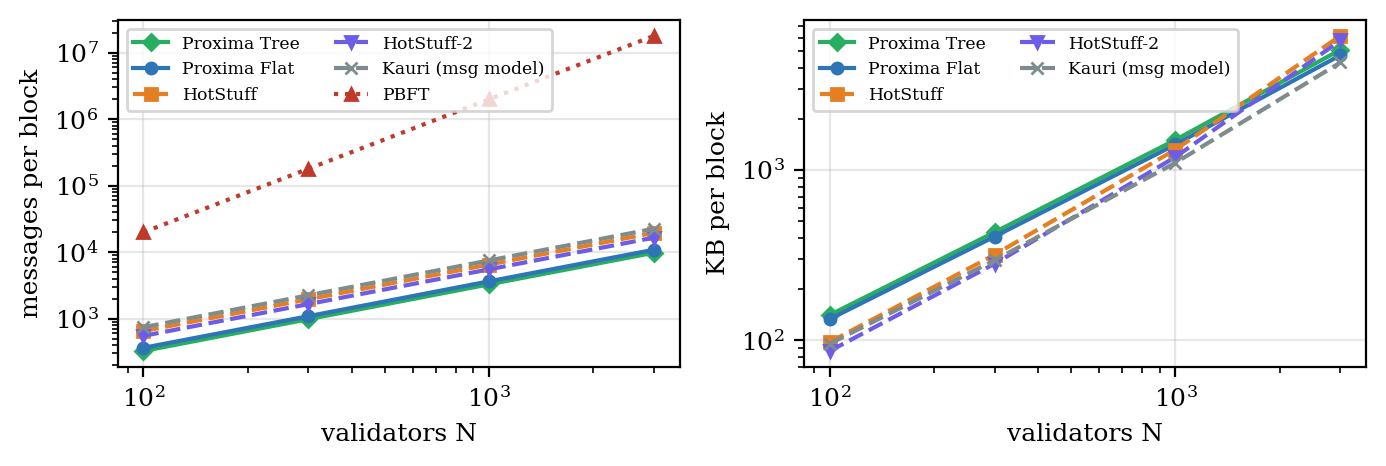
\includegraphics[width=\textwidth]{fig7_scaling.png}
\caption{Message (left) and bandwidth (right) scaling, log-log. Proxima
leads on messages throughout; on bandwidth the kilobyte digests cost a
premium at small $N$ that inverts beyond $N \approx 2000$ as
$\Theta(N^{2}/8)$ certificate bitmaps overtake $\Theta(N)$ digests.}
\label{fig:scaling}
\end{figure*}

\subsection{Fork Localization and Partition Healing}

Fig.~\ref{fig:forkheal} measures the accumulator machinery: fork
localization uses exactly $\log_{2} H + 1$ probes from $H = 64$ to
$H = 4096$ (7 to 13 probes, each one 2\,KB accumulator), with every probe
also reporting how much diverged; partition healing at 600-transaction
state recovers the exact union at sketch-plus-push cost tracking the
200-bytes-per-divergent-transaction floor, with the pre-repair estimate
$\hat{d}$ within its predicted error of the true divergence throughout.

\begin{figure*}[t]
\centering
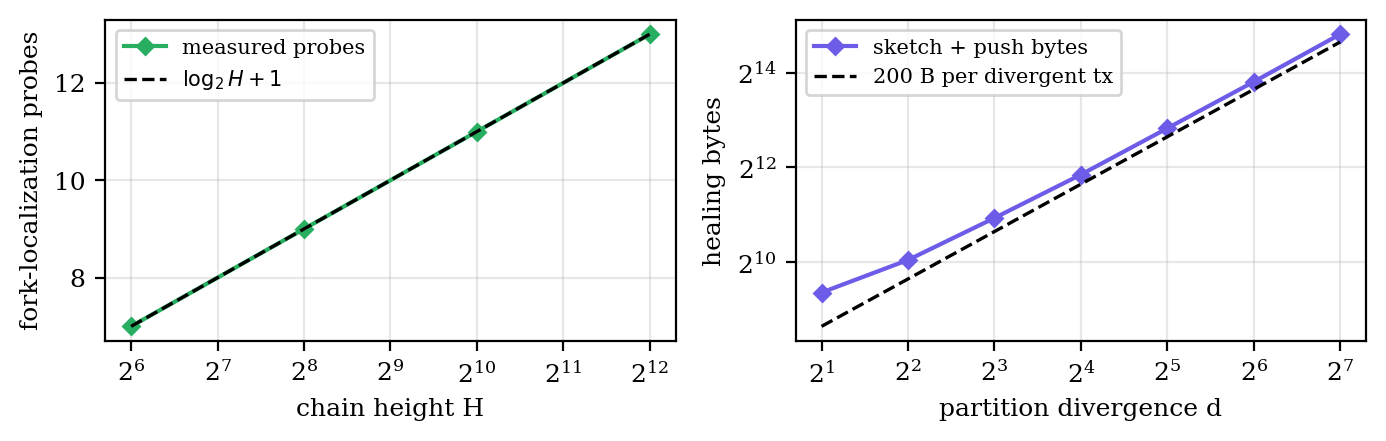
\includegraphics[width=\textwidth]{fig8_fork_heal.png}
\caption{Left: fork-localization probes against chain height, matching
$\log_{2} H + 1$ exactly. Right: partition-healing bytes against
divergence, tracking the per-transaction push floor.}
\label{fig:forkheal}
\end{figure*}

\subsection{What the Simulation Does Not Show}

Three honest limits bound these results. The Kauri numbers are a
message-count model that credits neither pipelining, Kauri's central
contribution to throughput, nor charges reconfiguration under relay
failure; a faithful comparison needs Kauri's own harness. Latency is not
reported at all: our earlier projections mixed measured constants with
modeled round trips, and we now regard a multi-region deployment as the
only honest source of latency claims (Section~\ref{sec:limits}). And
$p_{\mathrm{miss}} = 0.37$ remains an internal measurement; the sensing
results deliberately sweep it as a free parameter rather than defending
the point value.

%============================================================================
\section{Limitations and Future Work}
\label{sec:limits}

\textbf{Concrete cryptanalysis.} Binding rests on a reduction shape to a
$\pm 1$-matrix SIS instance plus first-cut Wagner and lattice estimates
and the inherited LtHash analysis; a dedicated cryptanalysis at exactly
our parameters ($n = 512$, $q \in \{2^{16}, 2^{32}\}$, block-bounded
weight) is open, and until it exists we claim no numeric security level.

\textbf{Deployment.} All numbers are simulation; a 50-to-200 node
deployment across three regions would convert message counts into
latency and throughput measurements and let us measure
$p_{\mathrm{miss}}$ rather than assume it.

\textbf{Adaptive adversaries.} The model is static corruption. An
adversary who corrupts after observing tree assignments or sensing
behavior requires VRF-based assignment with epoch rotation, described but
not evaluated here; note that Theorem~\ref{thm:compose} is indifferent to
this choice, since it holds against whatever adversary class $\Pi$
tolerates.

\textbf{Tree fast path.} Carrying speculative commitments up the tree
requires per-group signer bitmaps; the flat fast path does not extend
without them.

\textbf{Value semantics.} Conservation verifies multiset settlement, not
execution ordering; composing the invariant with an execution layer that
needs atomicity across more than two shards is future work.

%============================================================================
\section{Conclusion}
\label{sec:conclusion}

Collision-resistant hashing gives consensus protocols a one-bit view of
agreement, and the costs of that single bit run through the BFT
literature: mandatory synchronization, unmeasurable agreement, oversized
committees, per-transaction cross-shard coordination. The repair is not a
better hash but a division of labor that we prove is forced: estimation
objects cannot bind and binding objects cannot estimate, yet one
zero-mean additive multiset hash provides both faces, an unbiased
symmetric-difference estimator on its geometry and a SIS-hard homomorphic
accumulator on its equality. Around that object we rebuilt a BFT protocol
in which every optimistic mechanism fires on honest-sufficient conditions
and every estimate is repaired by an exact decoder, and we extended the
same algebra to sharded settlement as a conservation law with logarithmic
fraud localization. The composition theorem guarantees all of it costs
nothing in safety; the measurements say it pays in messages, in
robustness to griefing and reference manipulation, and, at scale, in
bandwidth.

\bibliographystyle{IEEEtran}
\bibliography{references}

\end{document}
